\chapter{Conclusioni e Lavoro Futuro}
\label{Conclusione}
%
Il modello sviluppato soddisfa il vincolo del tempo reale imposto per le simulazioni in tempo reale. Il tempo di calcolo sull'\textit{hardware} del simulatore professionale si traduce in un ciclo di lavoro del ??\%, garantendo quindi un ampio margine di sicurezza e dando la possibilità di aumentare la precisione del modello attraverso l'implementazione di modelli più complessi.

Dato che la rappresentazione dello pneumatico è basato sul modello di Pacejka, ovvero un modello semi-empirico, non tiene conto dei fenomeni transitori. Sarà quindi una scelta obbligata passare ad una rappresentazione dello pneumatico mediante un modello fisico. Quest'ultimo, infatti, a seconda del grado di complessità, può tenere in considerazione alcuni dei fenomeni transitori che maggiormente influenzano la manovrabilità del veicolo. I modelli fisici sono quindi anche molto complessi. Lo pneumatico è modellato da divesi anelli circolari con punti di massa accoppiati anche in direzione laterale. Si tiene quindi conto del contatto in più punti e della distribuzione della pressione su tutta la larghezza della cintura. Importante sarà quindi valutare la possibilità di poter parallelizzare i processi di calcolo per diminuire i tempi di esecuzione.

\begin{figure}
	\centering
	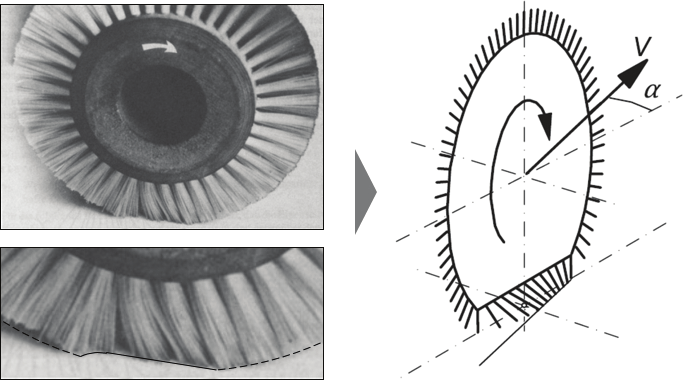
\includegraphics[width=0.7\linewidth]{Figures/brush_model}
	\caption{Schema strutturale del modello "a spazzola" (\textit{brush model}). }
	\label{brushmodel}
\end{figure}

Un punto critico sul quale è opportuno porre particolare attenzione è la rappresentazione del terreno. I \textit{file} \ac{RDF} hanno una struttura dati molto poco formale e solida. La mancanza di uno standard universalmente riconosciuto per questo formato rende impossibile implementare un \textit{parser} sufficientemente efficiente e la stabile per tutte le occasioni.

Infine, considerando le finalità principali di questa tesi e i test effettuati sul modello sviluppato, possiamo affermare la sua validità per i campi di utilizzo previsti.